\chapter{INTERFACE DESIGN}

\section{User Interface Characteristics}

Every user interface, whether designed for a Web application or a traditional software application, should exhibit the following characteristics:

\begin{itemize}
  \item \textbf{Easy to use:} The interface should be user-friendly and accessible.
  \item \textbf{Easy to learn:} Users should quickly understand how to navigate and use the system.
  \item \textbf{Easy to navigate:} Intuitive navigation enhances user experience.
  \item \textbf{Intuitive:} The interface should feel natural and be easy to understand.
  \item \textbf{Consistent:} Consistency in design elements helps users predict how the system behaves.
  \item \textbf{Efficient:} The system should allow users to accomplish tasks quickly and with minimal effort.
  \item \textbf{Error-free:} A well-designed interface minimizes the chances of user errors.
  \item \textbf{Functional:} The interface should serve its purpose effectively and meet user needs.
\end{itemize}

The Co-operative Society Management System follows all these principles of effective user interface design. Users can quickly see the breadth of their options, grasp how to achieve their goals, and do their work without being concerned with the inner workings of the system.

\section{SCREENSHOT OF THE SYSTEM}

\subsection{SYSTEM ENTRY SCREEN}
  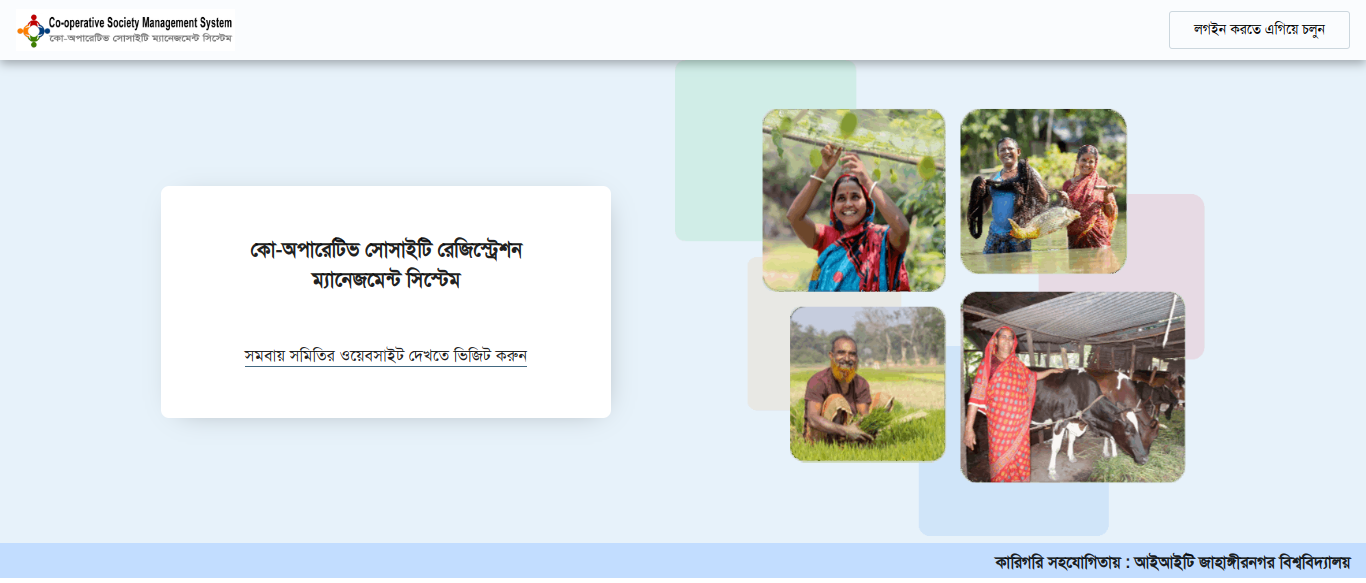
\includegraphics[width=14cm]{Chap4/1.png}

\subsection{Login Screen:}
  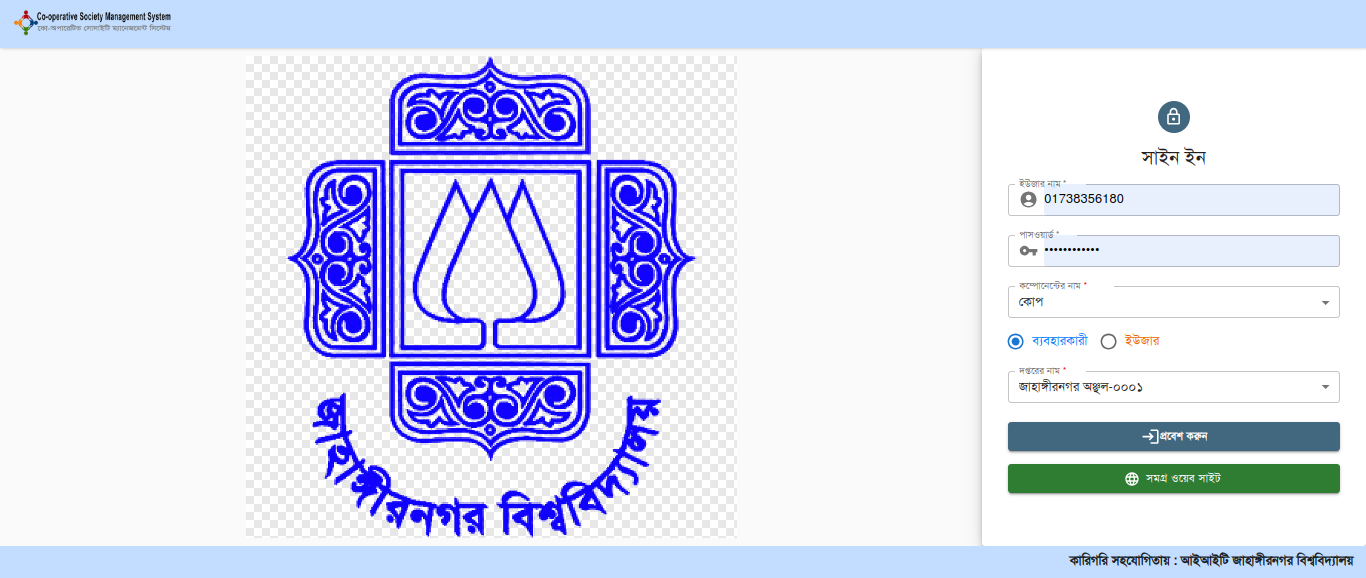
\includegraphics[width=14cm]{Chap4/2.png}
  
\subsection{User Dashboard:}
  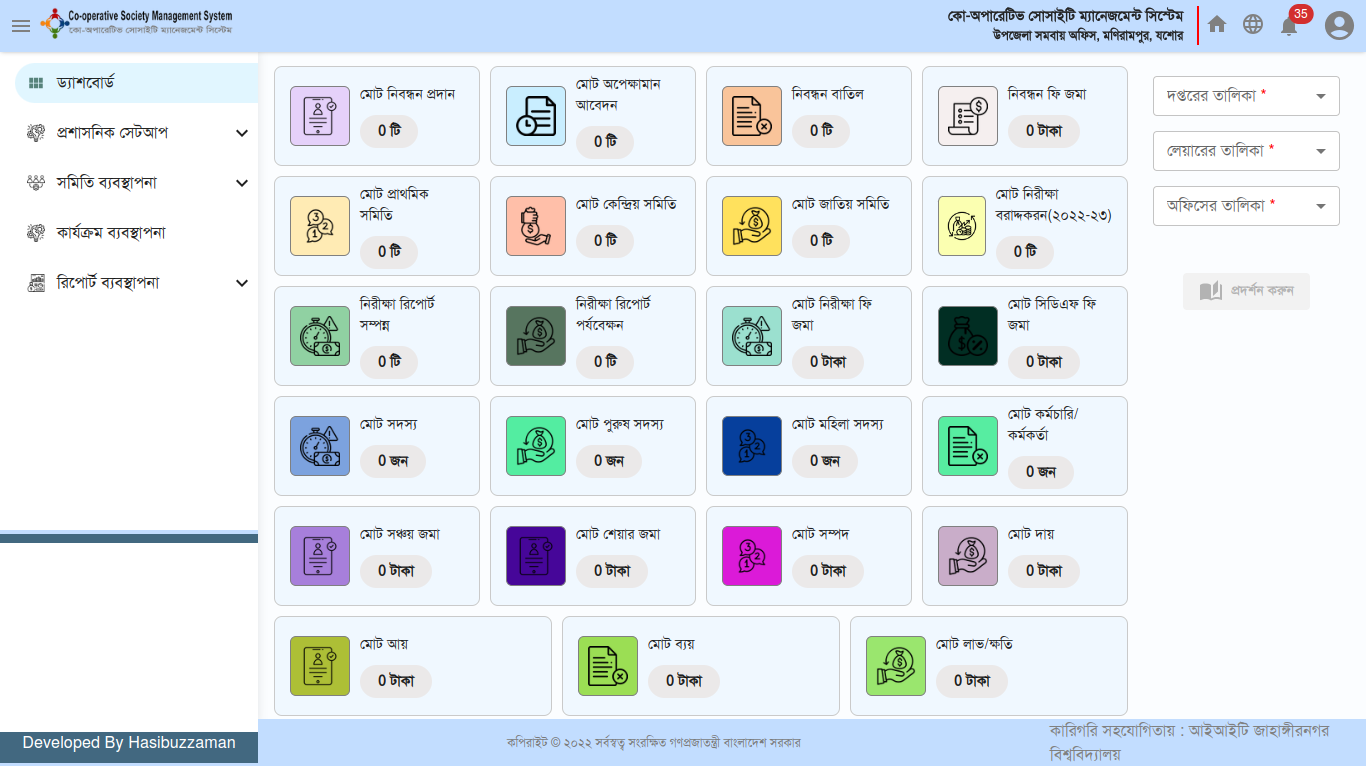
\includegraphics[width=14cm]{Chap4/3.png}

\subsection{Beneficiary Dashboard:}
  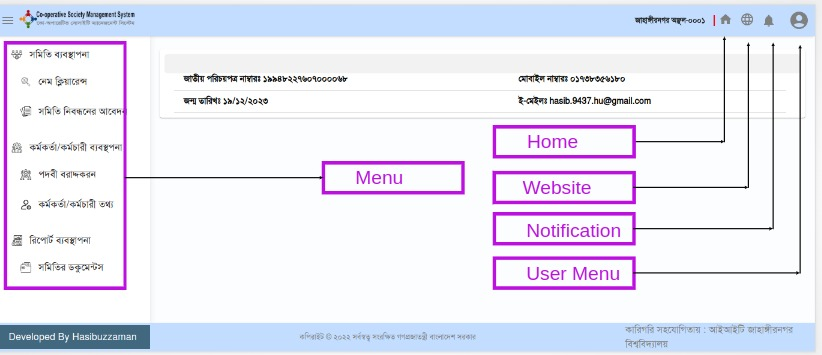
\includegraphics[width=14cm]{Chap4/4.jpeg}

\subsection{Name Clearance:}
  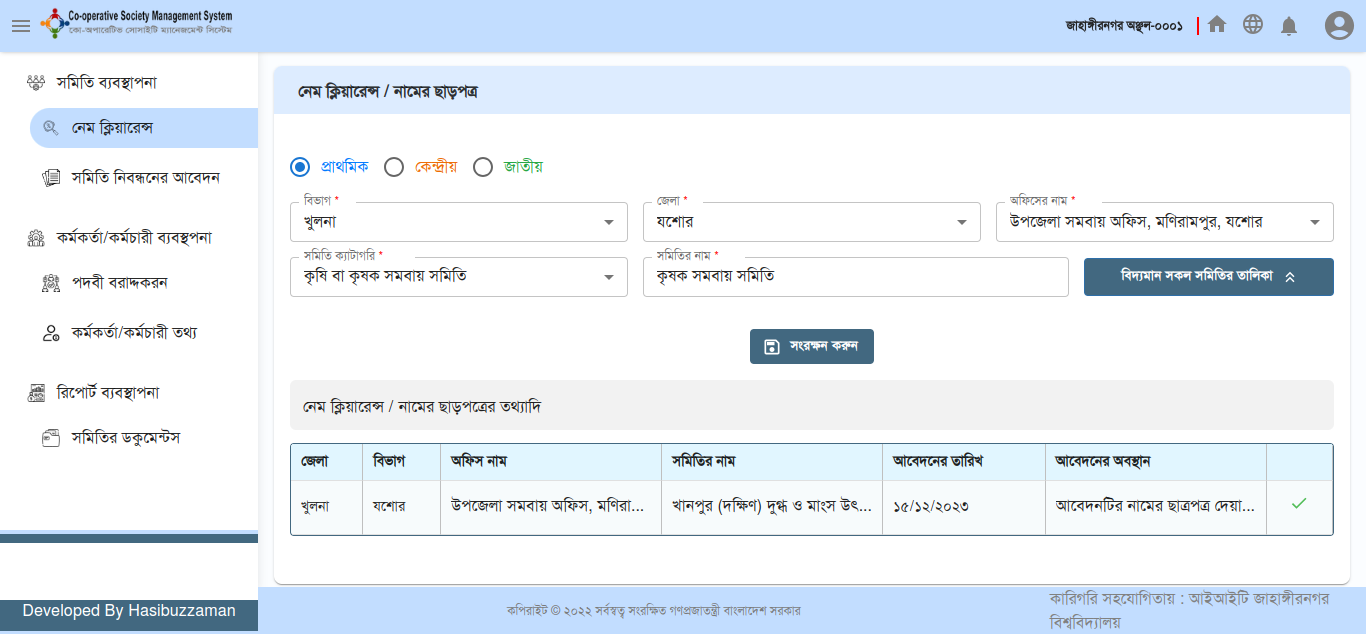
\includegraphics[width=14cm]{Chap4/5.png}

\subsection{Name Clearance:}
  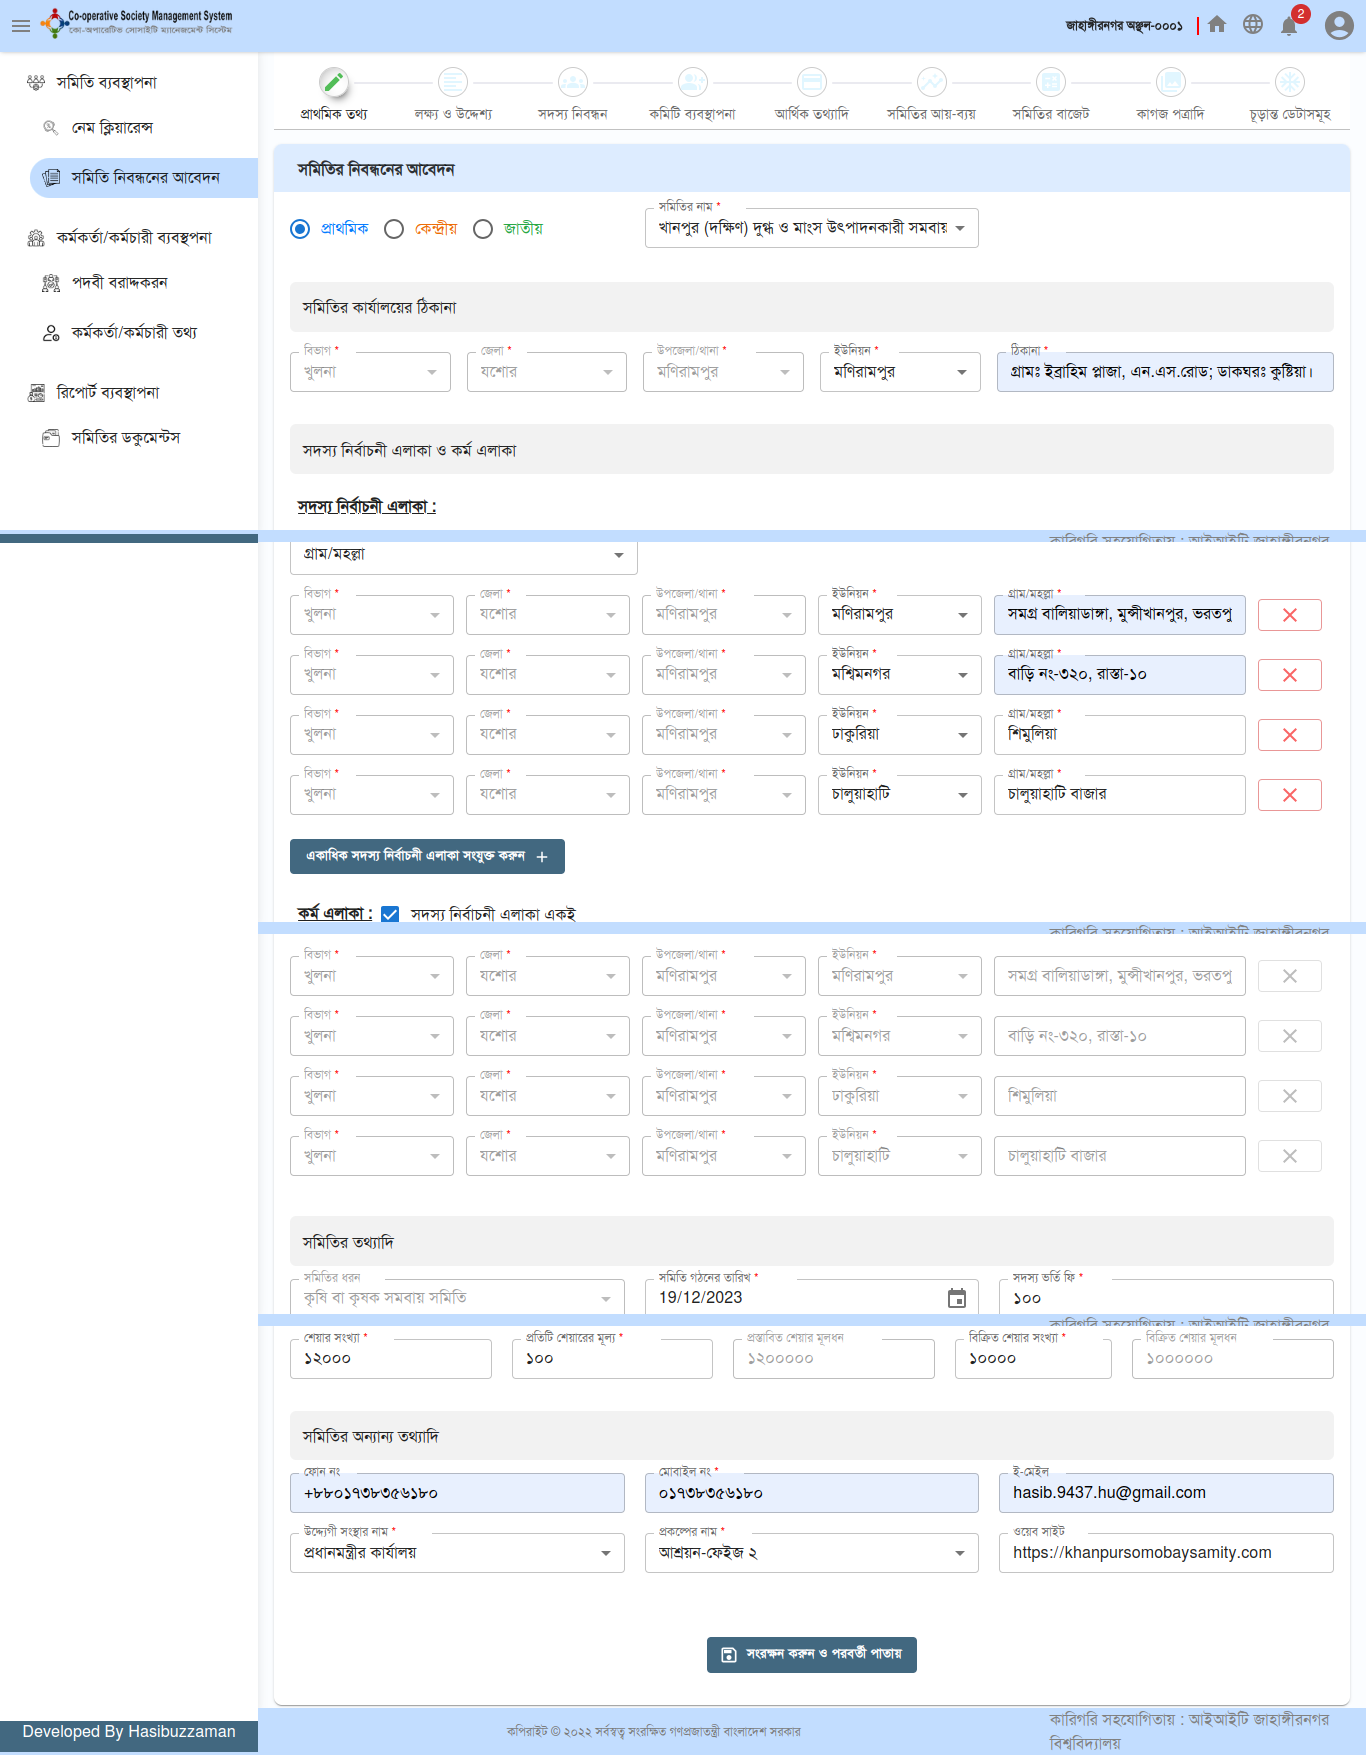
\includegraphics[width=14cm]{Chap4/6.png}